% PeerJ Computer Science, Research Article. Built 29 Sep 2026 from ../main_tmlr.tex; revised the
% same day after three reviews (see LAB-NOTEBOOK.md, 29 Sep 2026, revision entry).
% Format per https://peerj.com/about/author-instructions/cs (read 29 Sep 2026): US Letter, line
% numbers, 2.5 cm margins, 12 point Times, left-justified text, Author Cover Page first, abstract
% under 500 words, standard sections, declarations. A plain article class with those conventions;
% the official Overleaf template requires a PeerJ login to download. Stated in the cover letter.
\documentclass[12pt,letterpaper]{article}
\usepackage[margin=2.5cm]{geometry}
\usepackage[utf8]{inputenc}
\usepackage[T1]{fontenc}
\usepackage{mathptmx}
\usepackage{amsmath}
\usepackage{booktabs}
\usepackage{array}
\usepackage{graphicx}
\usepackage{xcolor}
\usepackage{url}
\usepackage{ragged2e}
\usepackage[labelfont=bf,justification=RaggedRight,singlelinecheck=false]{caption}
\usepackage[round,authoryear]{natbib}
\usepackage{lineno}
\usepackage[hidelinks]{hyperref}
\newcommand{\qtN}{400}
\newcommand{\qtSizeFp}{3.8}
\newcommand{\qtAccEight}{91.75}
\newcommand{\qtSizeEight}{2.2}
\newcommand{\qtAccSix}{93.50}
\newcommand{\qtSizeSix}{1.7}
\newcommand{\qtDeltaSix}{+1.75}
\newcommand{\qtLostSix}{6}
\newcommand{\qtGainedSix}{13}
\newcommand{\qtPSix}{0.167}
\newcommand{\qtAccFive}{90.75}
\newcommand{\qtSizeFive}{1.5}
\newcommand{\qtDeltaFive}{-1.00}
\newcommand{\qtLostFive}{10}
\newcommand{\qtGainedFive}{6}
\newcommand{\qtPFive}{0.454}
\newcommand{\qtAccFour}{92.00}
\newcommand{\qtSizeFour}{1.3}
\newcommand{\qtDeltaFour}{+0.25}
\newcommand{\qtLostFour}{13}
\newcommand{\qtGainedFour}{14}
\newcommand{\qtPFour}{1.000}
\newcommand{\qtAccThree}{87.00}
\newcommand{\qtSizeThree}{1.1}
\newcommand{\qtDeltaThree}{-4.75}
\newcommand{\qtLostThree}{30}
\newcommand{\qtGainedThree}{11}
\newcommand{\qtPThree}{0.004}
\newcommand{\qtSizeRatioFour}{59}
\newcommand{\qtCompressFour}{34}
\newcommand{\qtRepRunsEight}{3}
\newcommand{\qtRepMeanEight}{91.58}
\newcommand{\qtRepRangeEight}{0.25}
\newcommand{\qtRepListEight}{91.75, 91.50, 91.50}
\newcommand{\qtRepFlipsMaxEight}{1}
\newcommand{\qtRepRunsFour}{3}
\newcommand{\qtRepMeanFour}{91.83}
\newcommand{\qtRepRangeFour}{0.50}
\newcommand{\qtRepListFour}{92.00, 91.50, 92.00}
\newcommand{\qtRepFlipsMaxFour}{4}
\newcommand{\qtMaxRepRange}{0.50}
\newcommand{\qtCliffOverNoise}{10}
\newcommand{\qtRungsCount}{5}
\newcommand{\qtRunsTotal}{9}
\newcommand{\qtMacTg}{35}
\newcommand{\qtMacPp}{650}
\newcommand{\qtGcpTg}{22.0}
\newcommand{\qtGcpPp}{109.6}

\newcommand{\bfcl}{BFCL}
\newcommand{\qm}{Qwen3-1.7B}
\setlength{\parindent}{0pt}
\setlength{\parskip}{6pt plus 2pt}
\setlength{\bibsep}{4pt}
\raggedbottom

\title{Post-Training k-Quantization and Agentic Tool-Calling Accuracy on Five Qwen3 and Llama Models}
\author{Akshay Kumar}
\date{}

\begin{document}
\raggedright

% ---------------------------------------------------------------- Author Cover Page
\begin{titlepage}
\vspace*{2cm}
{\Large\bfseries Post-Training k-Quantization and Agentic Tool-Calling Accuracy on Five Qwen3 and Llama Models\par}
\vspace{1.5cm}
{\large Akshay Kumar$^{1}$\par}
\vspace{0.5cm}
$^{1}$ Independent Researcher\par
\vspace{1cm}
Corresponding author:\par
Akshay Kumar$^{1}$\par
Email address: akumar8@mt.iitr.ac.in\par
ORCID: 0009-0006-3613-538X\par
\vspace{1cm}
Article type: Research Article\par
Journal: PeerJ Computer Science\par
\vfill
\end{titlepage}

\linenumbers
\maketitle

\begin{abstract}
\textbf{Background.} Language models run on laptops after post-training quantization, and the format that ships is the llama.cpp k-quant. The accuracy cost of that compression has been measured on prose, knowledge and reasoning benchmarks, and not on the output an agent produces, which is a function call that a program then executes.

\textbf{Methods.} We built a five-rung k-quant ladder, Q8\_0 to Q3\_K\_M, from one FP16 source for \qm{}, and three-rung ladders for Qwen3-8B, Qwen3-14B, Llama-3.2-3B and Llama-3.1-8B. Every rung was scored on the Berkeley Function Calling Leaderboard's \texttt{simple\_python} category by deterministic syntax-tree matching ($n=\qtN{}$ or \qtNEightB{}), with a type-coerced secondary score, and on \qtLlamaThreeBGsmN{} GSM8K questions with the same weight files. Rungs are compared with McNemar's exact test on identical items, corrected within each model's family of tests by Holm's method; every accuracy and every paired difference carries a 95\% interval; two rungs were each run three times to measure the instrument. Five hypotheses with thresholds were written in a dated file on the first day; its first commit postdates the first ladder, so the study is not called pre-registered, and every departure from the file is tabulated.

\textbf{Results.} On \qm{} tool calling is flat from Q8\_0 through Q4\_K\_M and loses \qtDropThree{} points at Q3\_K\_M (Holm-adjusted $p=\qtPHolmThree{}$), about \qtCliffOverNoise{} times the run-to-run range. Free-form mathematics on those files loses \qtGsmDropThree{} points at that rung because \qtGsmTruncThree{} of 400 generations reach the 4{,}096-token budget while still reasoning; \qtGsmTruncCorrectThree{} of them commit to a correct answer first. Qwen3-8B and Qwen3-14B show no loss at any rung. Llama-3.2-3B loses \qtDropLlamaThreeBThree{} strict points at Q3\_K\_M (Holm $p=\qtPHolmLlamaThreeBThree{}$) and a suggestive \qtDropLlamaThreeBFour{} at Q4\_K\_M ($p=\qtPLlamaThreeBFour{}$, Holm \qtPHolmLlamaThreeBFour{}, one run); under the coerced verdict neither loss is detectable. Llama-3.1-8B's strict score rises from \qtAccLlamaEightBEight{}\% to \qtAccLlamaEightBThree{}\% down the ladder because its full-precision weights write numbers as quoted strings; scored on the parsed value, with \qtDecodeJsonLlamaEightBThree{} of its \qtDecodeErrLlamaEightBThree{} three-bit decode failures re-read as the well-formed JSON calls they are, it scores \qtCoercedAccLlamaEightBEight{}\%, \qtCoercedAccLlamaEightBFour{}\% and \qtCoercedAccLlamaEightBThree{}\%. A fair answer extractor moves the free-form numbers by at most \qtGsmGapMax{} points, and a logit penalty on overthinking markers changes tool-calling accuracy by \qtHfourDropThree{} points. The multi-turn arm is confounded: \qtMtCtxErrEight{}, \qtMtCtxErrFour{} and \qtMtCtxErrThree{} of 200 trajectories aborted on a server context limit shared by four slots.

\textbf{Conclusions.} At four bits no model shows a single-call loss larger than its paired interval allows: under the coerced verdict no lower interval end is below $\qtFourBitLoCoerced{}$ points and the minimum detectable difference is \qtFourBitMdeMin{} to \qtFourBitMdeMax{} points. At three bits \qm{} and, under strict scoring, Llama-3.2-3B lose accuracy; the other three models do not detectably. The length-driven collapse of chain-of-thought reasoning under three-bit weights does not reach a single tool call. A strict schema score can move in either direction under quantization because it also measures a formatting habit, and part of a checker's decode-failure count can be its own parser, so a coerced score and the failure types belong beside it.
\end{abstract}

\textbf{Keywords.} post-training quantization; llama.cpp; k-quant; tool calling; function calling; language model agents; BFCL; GSM8K; multiple comparisons

\section{Introduction}

A laptop runs \qm{} in its three-bit k-quant, Q3\_K\_M, as the model behind a small agent. The agent is asked to find the greatest common divisor of 36 and 48 and is handed one function to call, \texttt{number\_theory.gcd}. The same model at eight bits, Q8\_0, answers with the call \texttt{number\_theory.gcd(number1=36, number2=48)}. At three bits it answers with a sentence: ``The Greatest Common Divisor (GCD) of two numbers, say 36 and 48, is 24.'' The program waiting for a call receives prose, and the number in the prose is wrong as well; the answer is 12. Both outputs came from one FP16 weight file. Only the number of bits used to store each weight changed. This is item \texttt{simple\_python\_21} of the benchmark used below, one of \qtLostThree{} items the three-bit weights lose against the eight-bit weights, and the question of this paper is how often that happens, at which bit-width it starts, and whether the function call or the free-form reasoning breaks first.

The compression is post-training quantization \citep{dettmers2022int8,gptq2023,awq2024}. The full-precision file for \qm{} is \qtSizeFp{}\,GB; the version most people would run, Q4\_K\_M, is \qtSizeFour{}\,GB, about \qtCompressFour{}\% of it. The format nearly everyone uses on a laptop is the family of llama.cpp k-quants \citep{llamacpp}, because that is what Ollama and the desktop front ends serve, and a systematic review of language-model deployment on edge devices counts model compression, quantization included, as a central enabler of running these models on memory-limited hardware \citep{dincer2026edge}. Four bits is where the scaling analysis says the trade-off is best \citep{dettmers2023case,kumar2024precision}, and it is the default most front ends pull. Lower bit-widths are pursued for throughput as well as size, although \citet{malekar2025amdahl} show, for binary and ternary weights, that the throughput gain is capped by whatever part of the model stays in higher precision.

The cost of that compression has been measured with care, on tasks other than the one an agent performs. Broad evaluations cover language modelling, classification, knowledge, dialogue, long context and trustworthiness across many families \citep{jin2024comprehensive,li2024evaluating}; \citet{kurtic2024bf16} score the Llama-3.1 family under FP8, INT8 and INT4 on academic benchmarks and on chat, code-generation and long-context tasks; \citet{lee2024tradeoffs} score instruction-tuned models from 1B to 405B under four quantization methods on thirteen datasets; multilingual degradation has its own study \citep{marchisio2024multilingual}; long-context inputs lose up to 59\% under four-bit methods \citep{mekala2025longcontext}; reasoning models have been quantized and scored on mathematics and code \citep{liu2025quanthurts}. \citet{kurt2026quant} quantizes Llama-3.1-8B-Instruct into thirteen GGUF formats and scores each on GSM8K, HellaSwag, IFEval, MMLU, TruthfulQA and perplexity. \citet{lotfi2026overthink} measure five reasoning models under GPTQ, AWQ and FlatQuant on mathematics, code and science questions and find accuracy falling as chain-of-thought inflates. Every task in every one of these papers is free-form or multiple choice. None involves emitting a function call.

An agent calls tools \citep{patil2023gorilla,qin2023toolllm,yao2024taubench}. It emits a function name and a set of typed arguments that a program will execute. That output either passes the checker or it does not, with no partial credit and no reader to accept an approximate answer. Our starting intuition was that a function signature has none of the slack prose has, so compression should break tool calling at a higher bit-width than it breaks free-form accuracy. We wrote this down as our first hypothesis, with a threshold, in the hypothesis file described in \S\ref{sec:prereg}.

We built a controlled ladder, five k-quant formats produced from one FP16 source, and scored each rung on the Berkeley Function Calling Leaderboard \citep{bfcl2025}, which compares a model's call to a reference by deterministic abstract-syntax-tree matching; no model judges another model anywhere in the pipeline. We then ran each rung's file on a free-form control so that the two floors could be compared on identical parameters, repeated Q8\_0, Q4\_K\_M and Q3\_K\_M on four further models in two families, and re-scored every run under a checker that accepts a correctly valued argument in the wrong type.

For \qm{} the answer is the reverse of the one we expected. Tool-calling accuracy is flat from Q8\_0 through Q4\_K\_M and falls by \qtDropThree{} points at Q3\_K\_M, roughly \qtCliffOverNoise{} times the run-to-run noise of the instrument. On those files free-form mathematics falls by \qtGsmDropThree{} points at the same rung. Both floors sit between four and three bits, but the drop in tool calling is about an eighth of the drop in mathematics. The difference comes down to output length. At three bits the model's chain of thought \citep{wei2022cot} grows until \qtGsmTruncPctThree{}\% of math generations use up their token budget before reaching an answer. A tool call is a median of \qtToolNgenMedThree{} tokens at that rung, so the weights never get the room to wander. On Qwen3-8B and Qwen3-14B there is no cliff at any rung. On the Llama family the picture is different, and part of the difference is the checker rather than the weights: Llama-3.2-3B loses at three bits under strict scoring and not under coerced scoring, and Llama-3.1-8B's strict score rises under compression because its full-precision weights quote numbers, a habit the compressed weights partly lose (\S\ref{sec:family}).

\textbf{Contributions.} Each item names the table or figure that holds it.
\begin{enumerate}\setlength{\itemsep}{0pt}
\item A controlled k-quant ladder for tool calling: 5 rungs from one FP16 source on \qm{} ($n=\qtN{}$) and 3 rungs on 4 further models ($n=\qtNEightB{}$), scored by a deterministic checker and by a type-coerced secondary checker, with McNemar tests on identical items, Holm's correction within each model, Wilson 95\% intervals on every accuracy and an interval on every paired difference (\S\ref{sec:method}, Tables~\ref{tab:ladder} and~\ref{tab:models}).
\item An instrument measurement: identical weights re-run 3 times move by at most \qtMaxRepRange{} points and flip at most \qtRepFlipsMaxFour{} of \qtN{} verdicts (Table~\ref{tab:repeats}).
\item The \qm{} floor: no detectable loss down to Q4\_K\_M, then \qtDropThree{} points at Q3\_K\_M, Holm $p=\qtPHolmThree{}$, \qtLostThree{} lost against \qtGainedThree{} gained (Table~\ref{tab:ladder}); no loss at any rung on Qwen3-8B or Qwen3-14B (Table~\ref{tab:models}).
\item The free-form comparison on the same weight files: \qtGsmDropThree{} points at Q3\_K\_M with \qtGsmTruncThree{} of 400 generations at the 4{,}096-token budget, \qtGsmTruncCorrectThree{} of which commit to a correct answer before running on (Table~\ref{tab:gsm8k}, Figure~\ref{fig:ladder}); a 16{,}384-token re-run of those \qtBudOf{} items leaves \qtBudStillCapPct{}\% still at the cap.
\item A second family scored two ways: Llama-3.2-3B loses \qtDropLlamaThreeBThree{} strict points at Q3\_K\_M (Holm $p=\qtPHolmLlamaThreeBThree{}$) and \qtCoercedDropLlamaThreeBThree{} coerced points ($p=\qtCoercedPLlamaThreeBThree{}$); Llama-3.1-8B gains \qtDropLlamaEightBThree{} strict points at Q3\_K\_M and loses \qtCoercedDropLlamaEightBThree{} coerced points ($p=\qtCoercedPLlamaEightBThree{}$), with \qtCoercibleLlamaEightBEight{} of its \qtFailsLlamaEightBEight{} Q8\_0 strict failures being quoted values of the right number and \qtDecodeJsonLlamaEightBThree{} of its \qtDecodeErrLlamaEightBThree{} Q3\_K\_M decode failures being well-formed JSON calls that the harness's Python parser refuses (Tables~\ref{tab:models} and~\ref{tab:llama}).
\item A bound for four bits: on every model the paired Q8\_0 to Q4\_K\_M difference has a lower interval end no worse than $\qtFourBitLoCoerced{}$ points under the coerced verdict, and the minimum detectable difference at $n=\qtNEightB{}$ is \qtFourBitMdeMin{} to \qtFourBitMdeMax{} points (Table~\ref{tab:fourbit}).
\item Two null results: a fair extractor changes free-form accuracy by at most \qtGsmGapMax{} points at any rung (Table~\ref{tab:gsm8k}), and a logit penalty on overthinking markers changes tool-calling accuracy by \qtHfourDropThree{} points at Q3\_K\_M (\S\ref{sec:penalty}).
\item A multi-turn arm reported as confounded: \qtMtCtxErrEight{}, \qtMtCtxErrFour{} and \qtMtCtxErrThree{} of 200 trajectories aborted on a context limit shared by four server slots (Table~\ref{tab:multiturn}), so the multi-turn hypothesis is not evaluable from this run.
\end{enumerate}

\section{Related work}

\textbf{Quantization evaluated on free-form tasks.} The broad evaluations of post-training quantization score many model families on language modelling, multiple-choice knowledge, dialogue, long-context and trustworthiness tasks \citep{jin2024comprehensive,li2024evaluating}; a full-text search of both finds no tool-calling or function-calling benchmark. \citet{kurtic2024bf16} run more than half a million evaluations on the Llama-3.1 family under FP8, INT8 and INT4 and find FP8 effectively lossless, well-tuned INT8 1 to 3\% below the BF16 baseline, and INT4 weight-only quantization on par with 8-bit; \citet{lee2024tradeoffs} find quantized models generally ahead of smaller full-precision ones but weaker on instruction following and hallucination detection. Neither scores a function call. \citet{liu2025quanthurts} quantize the DeepSeek-R1-distilled and QwQ reasoning models and find mathematics and code degrading under aggressive weight and KV-cache quantization, again on free-form tasks. \citet{kurt2026quant} is the closest work and the one this paper extends: one model, thirteen llama.cpp formats from Q3\_K\_S to Q8\_0 against FP16, six free-form or multiple-choice benchmarks, plus throughput and size. A full-text read finds no tool-calling, function-calling, agentic, structured-output or schema-compliance evaluation, and its conclusion asks for exactly what we add, additional model families and sizes under the same protocol. \citet{lotfi2026overthink} take a different axis, in the line of work on overthinking in reasoning models \citep{chen2024overthinking,sui2025stop}. Under GPTQ \citep{gptq2023}, AWQ \citep{awq2024} and FlatQuant, five reasoning models lose accuracy while emitting longer chains of thought, and in up to 52\% of failures the correct answer appears mid-trace without being committed to. Their compression methods are research methods rather than the k-quants that ship to laptops, and their failure categorisation, including the overthinking class, relies on GPT-5 as a judge. Setting quantization aside, the gain from zero-shot chain-of-thought prompting over direct answering holds on average across six models and six question-answering datasets but varies in size by model and dataset \citep{hebenstreit2024cot}; what quantization does to the length of the chain is a further axis. Surveys of language models for constrained deployment list quantization among the standard compression techniques \citep{turkmen2026slm,dincer2026edge}, and the survey of small clinical models names agentic tool use as a future direction \citep{turkmen2026slm}; neither measures the two together.

\textbf{Tool-calling evaluation.} Gorilla \citep{patil2023gorilla} and ToolLLM \citep{qin2023toolllm} established API calling as a benchmark task, and $\tau$-bench \citep{yao2024taubench} extends it to multi-turn agent-user interaction. \bfcl{} \citep{bfcl2025} scores a model's function call against a reference by abstract-syntax-tree matching over the function name, argument names, types and values, across single, multiple and parallel calls, an irrelevance category where no call is correct, and multi-turn trajectories. Because the matcher is deterministic, the same generation always receives the same verdict, so a difference between two rungs can be attributed to the weights rather than to the scorer. \citet{dondeti2026toolguard} study the same class of small models on consumer hardware from the safety side, scoring adversarial tool calls from seven models between 1B and 4B parameters with a deterministic would-dispatch rule; this paper is the accuracy side of the same deployment.

\textbf{The gap.} Quantization has been scored on prose, knowledge, instruction following and reasoning, for research compression methods and for the deployed one. It has not been scored on tool calling under either. That is what we measure.

\section{Materials and Methods}
\label{sec:method}

\subsection{The hypotheses and their record}
\label{sec:prereg}
Five hypotheses with numerical thresholds are in \texttt{paper/preregistration.md} in the repository. The file is dated 18 September 2026 and, by the author's own record, was written that morning before the ladder was built. The repository cannot show that. The file's first commit, \texttt{cac7796} at 17:37:31 on 18 September 2026 (UTC$-$7), also contains the completed five-rung ladder, whose rungs finished between 14:33 and 15:23 that afternoon, both repeat arms (17:05) and a findings note. A second commit, \texttt{07cee6b} at 17:56, added the free-form extractor rules to the file's open-items list after 59 Q8\_0 generations had been read (\S\ref{sec:freeform-method}); no other line of the file has changed since, so the hypotheses and thresholds in the repository are those of the first commit, which the tag \texttt{prereg-v1} marks. Because no independent time stamp precedes the first results, we do not call the study pre-registered. What we do instead: each hypothesis is evaluated against the threshold the file states (\S\ref{sec:hyp}); the statistics, which the file does not name, are labelled as choices made after the first run (\S\ref{sec:problem}); and Table~\ref{tab:deviations} lists every departure from the design the file describes.

\begin{table}[p]
\centering\footnotesize
\begin{tabular}{@{}p{2.6cm}p{4.2cm}p{4.6cm}p{4.6cm}@{}}
\toprule
Item & Planned in the file & Done & Why \\
\midrule
Reference arm & FP16 & Q8\_0; no FP16 rung was run & No reason was recorded. Every comparison is against Q8\_0. \\
Models & DeepSeek-R1-Distill-Qwen 1.5B and 7B; Qwen3 1.7B, 4B, 8B and 14B; Llama-3.1-8B & Qwen3-1.7B, 8B and 14B; Llama-3.1-8B; Llama-3.2-3B added & \texttt{bfcl-eval} has no model entry for the R1-Distill checkpoints (notebook, 19 Sep) nor for the original Qwen3-4B, only for a later lineage (18 Sep). Llama-3.2-3B was added on 25 Sep as a second model in the 1.7B size band. \\
\bfcl{} subsets & Non-live, live and multi-turn, reported separately & \texttt{simple\_python} on all five models; \texttt{multi\_turn\_base} on \qm{} & Compute was spent in the order free-form control, penalty arm, larger models, multi-turn (notebook, 18 Sep); the live categories were never queued. \\
Metrics & AST accuracy; schema validity; hallucinated-function rate; type-error rate; output length; latency & AST accuracy, type errors and output length as planned; schema validity, hallucinated-function rate and structural share added in this revision (\S\ref{sec:hyp}); latency for the \qm{} ladder only & The other models ran in sleep-interrupted nightly windows (notebook, 26 Sep), so their wall-clock times are not a property of the model. \\
H1 statistic & Schema validity below 95\% of the reference & Reported as written (it never triggers) and on AST accuracy & With no decode failures on \qm{}, schema validity has almost no variance. \\
H2 threshold & Structural share of failures up by 15 points & Computed in this revision (Table~\ref{tab:htwo}) & Not computed in earlier drafts. \\
H3 statistic & AST drop smaller than the strict free-form drop by 5 points & Reported as written (supported); the strict-minus-lenient gap reported separately & Earlier drafts scored H3 on the extractor gap, a different quantity. \\
Statistical tests & None named & McNemar's exact test, Wilson intervals, $\alpha=0.05$ and the cliff rule; Holm's correction, paired intervals and minimum detectable differences & The first four chosen on the evening of 18 Sep after the first ladder; the rest added after review. \\
Extra arms & Not in the file & Repeat runs; the 16{,}384-token budget re-run; the coerced verdict; the penalty at two rungs & Added as the results raised them. \\
Free-form extractor & Strict regex; lenient hierarchical & Strict widened to the boxed form after 59 Q8\_0 generations were read (\texttt{07cee6b}, 17:56) & The first rule was a strawman; the gap it would have produced is not reported. \\
Hardware & M1 Pro, 16\,GB & M1 Max, 64\,GB & The machine had more memory than assumed at planning (notebook, 18 Sep). \\
Working title & Asserted H1 & Changed & H1 reversed. \\
\bottomrule
\end{tabular}
\caption{Every departure from the design in \texttt{paper/preregistration.md}. Dates refer to the lab notebook in the repository.}
\label{tab:deviations}
\end{table}

\subsection{Problem statement}
\label{sec:problem}
A \emph{ladder} for a model $M$ is an ordered list of weight files $r_0, r_1, \dots, r_K$ produced from one FP16 source with one quantizer, in decreasing bits per weight, so that the files differ in their weights and in nothing else. Here $r_0$ is always Q8\_0. An \emph{item set} $I$ is a fixed list of $n$ benchmark items with reference answers. A \emph{verdict} $v(i, r) \in \{0, 1\}$ is the deterministic output of a checker on the model's response to item $i$ served from rung $r$, and \emph{accuracy} $A(r)$ is the mean verdict over $I$. Two verdict functions are used for tool calling. The \emph{strict} verdict is \bfcl{}'s abstract-syntax-tree match. The \emph{coerced} verdict equals the strict verdict except that a strict failure is re-checked by the same checker after every string-typed argument whose schema declares a non-string type is replaced by its parsed value when it parses as that type, and after an output the handler could not decode is re-read as JSON when it is one well-formed call (\S\ref{sec:scoring}); a quoted number, list or boolean counts when the parsed value is what the reference holds and not otherwise. The coerced verdict is never below the strict one.

Rungs are compared to $r_0$ pairwise on the same items. The test is McNemar's exact test on the discordant pairs \citep{mcnemar1947}: \emph{lost} counts items with $v(i, r_0)=1$ and $v(i, r)=0$, \emph{gained} the reverse, and $p$ is the two-sided exact binomial probability of a split at least that uneven under the null of no difference. Tests are grouped into families and corrected within each family by Holm's step-down method \citep{holm1979}. A family is every distinct McNemar test against one model's Q8\_0 on the single-call arm, under both verdicts; for the Qwen3 models the coerced verdicts equal the strict ones, so the family has one test per rung (\qtTests{} for \qm{}, \qtTestsEightB{} each for Qwen3-8B and Qwen3-14B), and for the Llama models two per rung (\qtTestsLlamaThreeB{} each). The free-form arm of each model, the multi-turn arm and the penalty arm are families of their own. The paper reports \qtTestsTotal{} tests in \qtFamiliesTotal{} families, and every table gives the raw $p$ with the Holm-adjusted $p$ in brackets. Every accuracy carries a Wilson score 95\% interval, in square brackets, and every paired difference carries the adjusted Wald 95\% interval of \citet{agresti2005paired}. The \emph{cliff rung} $c(M)$ is the highest-precision rung $r_k$, $k \ge 1$, with $A(r_k) < A(r_0)$ and Holm-adjusted $p < 0.05$ against $r_0$. The \emph{floor} is the rung immediately above the cliff rung, the lowest-bit rung on the ladder with no detected loss. A model is \emph{flat} on the ladder when it has no cliff rung, so its floor is at or below the lowest rung measured. A detected loss must also exceed the \emph{instrument tolerance} $\tau$, the largest range in accuracy across three runs of identical weights and settings (\S\ref{sec:repro}); on this instrument $\tau = \qtMaxRepRange{}$ points, and every loss reported as a cliff below is at least \qtCliffOverNoise{} times larger. The test, the interval, $\alpha$ and the cliff rule were chosen on the evening of 18 September 2026, after the first ladder had run and not in the hypothesis file; the Holm correction and the paired intervals were added after review.

``No detectable loss'' has a size. For each model at Q4\_K\_M, Table~\ref{tab:fourbit} gives the \emph{minimum detectable difference}: the smallest paired loss McNemar's test would detect at $\alpha=0.05$ with 80\% power at the discordance rate observed on that model, from the sample-size formula of \citet{connor1987paired} solved for the difference. At $n=\qtNEightB{}$ and the discordance seen here it is \qtFourBitMdeMin{} to \qtFourBitMdeMax{} points under the coerced verdict, so a loss of three points on an $n=\qtNEightB{}$ model is inside what this design cannot exclude, and every ``no detectable loss'' below should be read with that bound beside it. Item counts are $n=\qtN{}$ for the \qm{} ladder and both free-form arms, and $n=\qtNEightB{}$ for the other four models and for the multi-turn category, which has \qtMtN{} items in all. Every rung is a single run except the two \qm{} rungs used for the tolerance measurement, so a stranger who repeats one rung should expect its accuracy to move within $\tau$ and its verdicts on a few items to flip.

Under these definitions the cliff rung is \qtCliffStrict{} for \qm{} under both verdicts, \qtCliffStrictEightB{} for Qwen3-8B and \qtCliffStrictFourteenB{} for Qwen3-14B (both flat), \qtCliffStrictLlamaThreeB{} strict and \qtCliffCoercedLlamaThreeB{} coerced for Llama-3.2-3B, and \qtCliffStrictLlamaEightB{} for Llama-3.1-8B under either verdict. The Results section gives the numbers behind each.

\subsection{The ladder}
Every rung of \qm{} \citep{qwen3} is produced from a single FP16 GGUF with \texttt{llama-quantize}. The formats are a subset of the ladder in \citet{kurt2026quant}, chosen to span the range at one rung per bit-width: Q8\_0, Q6\_K, Q5\_K\_M, Q4\_K\_M and Q3\_K\_M. Ollama's library publishes only two of these five for this model, Q8\_0 and Q4\_K\_M, alongside FP16, which is why the ladder is built rather than pulled. A Qwen3-4B rung was planned and dropped: \texttt{bfcl-eval} has no entry for the original Qwen3-4B, only for the later Instruct-2507 lineage, and mixing lineages would have confounded the size comparison. Four further models get three rungs, Q8\_0, Q4\_K\_M and Q3\_K\_M: the top of the ladder, the default most front ends pull, and the first rung below it. Each is built from its own FP16 source with the same quantizer: Qwen3-8B and Qwen3-14B from the same family, and Llama-3.2-3B-Instruct and Llama-3.1-8B-Instruct from a second family, whose Llama 3.1 models are described in \citet{llama3}. The FP16 sources are the \texttt{*-fp16} blobs Ollama distributes. Per model the design is: \qm{}, 5 rungs, $n=\qtN{}$, with 3 runs at Q8\_0 and Q4\_K\_M; Qwen3-8B, Qwen3-14B, Llama-3.2-3B and Llama-3.1-8B, 3 rungs each, $n=\qtNEightB{}$, 1 run per rung. Both Llama models are instruction-tuned rather than reasoning-tuned, which is deliberate: it separates what the ladder does to a tool call from what it does to a chain of thought. Llama-3.1-8B-Instruct is also the model \citet{kurt2026quant} quantized, so the two ladders meet on one model.

\subsection{Serving}
\label{sec:serving}
Each rung is served by \texttt{llama-server} from llama.cpp (the binary reports version 0.4.1, build 10964, commit b29c606e2; Homebrew) with full Metal offload on an Apple M1 Max with 64\,GB of memory, under a fixed model alias, so the harness sends identical requests to every rung. The single-call ladder and the repeats use \qtLadderSlots{} slots and an \qtLadderCtx{}-token context; the free-form control, the larger models, the Llama models and the multi-turn runs use \qtMtCtxSlot{}, because reasoning traces overflowed the smaller context; the 16{,}384-token budget re-run uses 65{,}536 with two slots. In every configuration the KV cache is one buffer shared by the slots (\texttt{kv\_unified}), so concurrent requests share the context figure rather than each owning it. A single call has a median prompt of \qtToolInMedEight{} tokens and a median completion of \qtToolNgenMedThree{} to \qtToolNgenMedEight{} tokens (\S\ref{sec:freeform}), so the context setting cannot affect the single-call arms, and the cross-model comparison in Table~\ref{tab:models} is unaffected by the two settings it mixes. It does affect the multi-turn arm, where trajectories accumulate a median context of \qtMtCtxMedEight{} to \qtMtCtxMedThree{} tokens per request and four of them together overflow the shared cache (\S\ref{sec:multiturn}). Generation is at temperature 0.001, the \texttt{bfcl-eval} default, for both arms. No sampling seed is fixed: \texttt{llama-server} is run with its default seed of $-1$, which draws a fresh random seed per request, so decoding is near-greedy but not bit-identical between runs. The repeat control below measures what that leaves. For the tool-calling arm, \texttt{bfcl-eval} 2026.3.23 builds the prompt itself in each model's own function-calling format and sends it to the server's raw completions endpoint, so the server's \texttt{-{}-jinja} chat template is not involved in those runs; the free-form arm uses the chat completions endpoint, where the template applies. Throughput, recorded in the lab notebook rather than computed from the logs, is about \qtMacTg{} tokens per second per slot and \qtMacPp{} tokens per second of prompt evaluation; the median latency of a single call on the \qm{} ladder, from the result files, is \qtToolLatMedEight{} to \qtToolLatMedFour{}\,s. Python is 3.12.

\subsection{Scoring}
\label{sec:scoring}
\bfcl{} v4 \citep{bfcl2025}, \texttt{simple\_python} category, deterministic AST matching, run through the \texttt{-FC} handler of each model so that the model uses its native function-calling format. The strict verdict is the checker's own. The coerced verdict is computed afterwards from the score files, with no new generation: each strict failure is passed back through \bfcl{}'s \texttt{simple\_function\_checker} with string arguments parsed to the type the function schema declares (\texttt{analysis/coerced.py} in the repository). A quoted integer is parsed only if it is an integer literal, a quoted list only if it parses as a list, a quoted boolean only if it is \texttt{true} or \texttt{false}; anything else is left as the string it was, and the checker then compares the parsed value with the reference exactly as it would a natively typed one, including nested types and optional parameters. One further step was added in this revision after reading the raw outputs behind the Llama-3.1-8B decode failures (\S\ref{sec:family}): \texttt{bfcl-eval}'s Llama 3.1 handler decodes a single call with Python's \texttt{eval()}, which refuses the JSON literals \texttt{true}, \texttt{false} and \texttt{null} that Meta's tool-call format allows. A strict decode failure whose raw output \texttt{json.loads()} reads as exactly one \texttt{\{"name": ..., "parameters": \{...\}\}} object is treated as that call and checked like any other; anything else stays a decode failure. The Qwen3 runs are unchanged by either step: \qtCoercibleQwenTotal{} of their \qtFailsQwenTotal{} strict failures across all rungs are of the coercible kind and \qtDecodeQwenTotal{} are decode failures. Differences between rungs are tested with McNemar's exact test on the discordant pairs, corrected within families, and every accuracy carries a Wilson 95\% interval, as defined in \S\ref{sec:problem}.

\subsection{Reproducibility control}
\label{sec:repro-method}
Two rungs of \qm{}, Q8\_0 and Q4\_K\_M, were run three times each with the same weights and settings. This gives the run-to-run variation of the instrument, which is needed before any difference between rungs can be read as a difference between weights. The control was run on the 1.7B model only; the other four models are single runs and inherit its tolerance as an assumption, which the Limitations section returns to.

\subsection{Free-form control}
\label{sec:freeform-method}
The same five \qm{} weight files, and the three files of each Llama model, answer 400 GSM8K test questions \citep{gsm8k2021}, drawn at seed 42, through the same server under the same alias, with a 4{,}096-token completion budget. Every generation is logged in full so that scoring under a different extractor is a re-read rather than a re-run. Two extractors are used. Strict accepts an explicit commitment in any of three forms, ``The answer is $N$'', ``\#\#\#\# $N$'', or $\backslash$boxed$\{N\}$, and takes the last such commitment in the text, so a boxed number mid-trace followed by a later ``The answer is'' yields the later one. Lenient takes the last number in the visible answer. Our first strict rule accepted only the first form; on the first 59 Q8\_0 generations it would have scored 21 wrong for writing the answer in a box. That rule was a strawman, it was replaced before any rung was scored (commit \texttt{07cee6b}, 18 September, 17:56), and the gap it would have produced is not reported anywhere in this paper.

\subsection{Check against the published leaderboard}
\label{sec:sanity}
Llama-3.1-8B-Instruct at Q8\_0 scores \qtAccLlamaEightBEight{}\% under the strict checker here, which is far below what the public leaderboard reports for that model, so the comparison is stated before the results. The \bfcl{} leaderboard data file \citep{bfclleaderboard2026}, last modified \qtBfclDataDate{} and retrieved on \qtBfclFetchDate{}, lists Llama-3.1-8B-Instruct in prompting mode only, as ``Llama-3.1-8B-Instruct (Prompt)'', at \qtBfclPromptPySimple{}\% on Python simple AST over the full 400 items; it lists no function-calling row for the model (\qtBfclLlamaFcRows{} of its \qtBfclLlamaRows{} Llama-3.1-8B rows). Our run uses the function-calling handler, in which \texttt{bfcl-eval} builds Meta's JSON tool-call prompt for Llama 3.1 itself and sends it to the raw completions endpoint of \texttt{llama-server}. The \texttt{meta-llama} repositories are gated, so the tokenizer and configuration are loaded from the ungated mirrors \texttt{unsloth/Llama-3.1-8B-Instruct} (snapshot \texttt{4699cc75}, \texttt{tokenizer\_config.json} SHA-256 \texttt{671ecdff\ldots{}3465}, \texttt{config.json} \texttt{ad98082c\ldots{}928b}) and \texttt{unsloth/Llama-3.2-3B-Instruct} (snapshot \texttt{006f5dcd}, \texttt{tokenizer\_config.json} \texttt{9ddd255c\ldots{}7458}); the full hashes are in the lab notebook, and the environment variables are \texttt{REMOTE\_OPENAI\_BASE\_URL} and \texttt{REMOTE\_OPENAI\_TOKENIZER\_PATH} in \texttt{run\_llama.sh}. In that format the full-precision model writes numeric arguments as quoted strings, which the strict checker rejects, and the handler's \texttt{eval()} refuses a bare JSON boolean (\S\ref{sec:scoring}). The coerced score at Q8\_0, \qtCoercedAccLlamaEightBEight{}\% [\qtCoercedCiLlamaEightBEight{}] on the first \qtNEightB{} items, is consistent with the published prompting-mode number, so the gap between \qtAccLlamaEightBEight{}\% and \qtBfclPromptPySimple{}\% is the argument-typing habit under the JSON tool-call format as read by this handler, not the weights or the server. A cross-check of the same GGUF files through a second path that renders Meta's tool template itself (the chat completions endpoint with \texttt{-{}-jinja} and a \texttt{tools} field) has not been run; the Limitations section lists it first.

\subsection{Overthinking penalty}
\citet{lotfi2026overthink} report that a fixed logit penalty on a curated list of overthinking markers cuts chain-of-thought length by 12 to 23\% while preserving accuracy. We apply a fixed penalty of $-2.0$ to the eight Qwen3 tokens for \emph{wait}, \emph{but}, \emph{alternatively} and \emph{hmm} in both capitalisations, at the server, and re-run the \qm{} ladder at Q4\_K\_M and Q3\_K\_M. This approximates their method with a single fixed $\lambda$ rather than their tuned value.

\subsection{Reproducibility}
Every number in this paper is a macro recomputed from the raw \bfcl{} result and score files, the logged generations, the server logs and the Ollama manifest of the FP16 source, with one exception: the throughput figures in \S\ref{sec:serving} are recorded from the lab notebook. The scripts, all in the repository named in the Data Availability statement, are: \path{analysis/paper_numbers.py}, which writes \path{paper/tables/numbers.tex} and every table from \path{runs/}; \path{analysis/coerced.py}, the coerced re-score and the failure classification; \path{analysis/figure.py}, Figure~\ref{fig:ladder}; \path{run_ladder.sh}, which rebuilds the \qm{} ladder from the FP16 source and scores it; \path{run_model.sh}, which does the same for Qwen3-8B, Qwen3-14B and the multi-turn category; \path{run_llama.sh} and \path{run_gsm8k_model.sh}, which build and score the two Llama models on both arms; and \path{run_repeats.sh}, \path{run_gsm8k.sh}, \path{run_budget.sh} and \path{run_h4.sh} for the reproducibility, free-form, budget and penalty arms. The GGUF weight files are not in the archive; \path{run_ladder.sh} and \path{run_model.sh} rebuild them from the published FP16 checkpoints.

\section{Results}

\subsection{The instrument is reproducible}
\label{sec:repro}

Table~\ref{tab:repeats} gives three runs of two rungs with the same weights and settings. Q8\_0 moved by \qtRepRangeEight{} points across three runs and Q4\_K\_M by \qtRepRangeFour{}. At the level of individual questions, at most \qtRepFlipsMaxEight{} of \qtN{} verdicts changed between two Q8\_0 runs and at most \qtRepFlipsMaxFour{} between two Q4\_K\_M runs. The instrument is close to deterministic, so any difference between rungs larger than about \qtMaxRepRange{} points can be attributed to the weights rather than to run-to-run variation.

\begin{table}[t]
\centering\footnotesize\setlength{\tabcolsep}{4pt}
\begin{tabular}{@{}llrr@{}}
\toprule
Rung & Accuracy per run & Range (pp) & Max per-question flips \\
\midrule
Q8\_0 & 91.75, 91.50, 91.50 & 0.25 & 1 of 400 \\
Q4\_K\_M & 92.00, 91.50, 92.00 & 0.50 & 4 of 400 \\
\bottomrule
\end{tabular}

\caption{Run-to-run variation with the same weights and settings, \qm{}, \texttt{simple\_python}, $n=\qtN{}$.}
\label{tab:repeats}
\end{table}

\subsection{Flat to four bits, a cliff at three}
\label{sec:ladder}

Table~\ref{tab:ladder} is the ladder. From Q8\_0 down to Q4\_K\_M the accuracy sits in a band of under three points and no rung differs from Q8\_0 at any conventional level: Q4\_K\_M is at \qtAccFour{}\% [\qtCiFour{}] against Q8\_0's \qtAccEight{}\% [\qtCiEight{}], a difference of \qtDeltaFour{} points \qtDiffCiFour{} with a McNemar $p$ of \qtPFour{}, while being \qtSizeRatioFour{}\% of the file size. Q6\_K scores above Q8\_0 and Q5\_K\_M below it, and neither difference survives paired testing, so the apparent non-monotonicity in the raw numbers is within the instrument's noise.

Q3\_K\_M is a different case. It loses \qtLostThree{} questions that Q8\_0 gets right and recovers \qtGainedThree{}, a net loss of \qtDropThree{} points \qtDiffCiThree{} at $p=\qtPThree{}$, Holm-adjusted \qtPHolmThree{} within the four tests of this ladder. That drop is about \qtCliffOverNoise{} times the largest run-to-run range in Table~\ref{tab:repeats}, which places the tool-calling floor for this model at Q4\_K\_M and the cliff rung at Q3\_K\_M. Of the \qtLostThree{} lost items, \qtLostThreeValue{} are calls with a wrong argument value and \qtLostThreeType{} has a wrong type; \qtLostThreeNoCall{} emit no call at all, either prose in place of a call, as in the GCD item of the introduction, or a trace that never reaches the call, which \bfcl{}'s Qwen handler decodes as an empty call list and scores as a wrong call count rather than a decode failure; \qtLostThreeName{} name a corrupted version of the right function.

\begin{table}[t]
\centering\footnotesize\setlength{\tabcolsep}{4pt}
\begin{tabular}{@{}lrrrrrr@{}}
\toprule
Rung & Size (GB) & Accuracy & vs.\ Q8\_0 & Lost & Gained & McNemar $p$ \\
\midrule
Q8\_0 & 2.2 & 91.75\% & baseline & & & \\
Q6\_K & 1.7 & 93.50\% & $+$1.75\,pp & 6 & 13 & 0.167 \\
Q5\_K\_M & 1.5 & 90.75\% & $-$1.00\,pp & 10 & 6 & 0.454 \\
Q4\_K\_M & 1.3 & 92.00\% & $+$0.25\,pp & 13 & 14 & 1.000 \\
Q3\_K\_M & 1.1 & 87.00\% & $-$4.75\,pp & 30 & 11 & \textbf{0.004} \\
\bottomrule
\end{tabular}

\caption{The quantization ladder for \qm{} on \texttt{simple\_python}, $n=\qtN{}$ per rung, all rungs from one FP16 source, one run per rung. Brackets after an accuracy are Wilson 95\% intervals. Lost and gained count questions that flip against Q8\_0; $p$ is McNemar's exact test on those discordant pairs, followed by the Holm-adjusted $p$ within this ladder's four tests, in bold where the adjusted value is below 0.05.}
\label{tab:ladder}
\end{table}

\subsection{The free-form floor on the same weights}
\label{sec:freeform}

Figure~\ref{fig:ladder} puts both tasks on one axis and Table~\ref{tab:gsm8k} gives the numbers. The tool-calling line barely moves while the free-form line drops sharply at the same rung, and the right panel shows the reason. The free-form floor sits exactly where the tool-calling floor sits, at Q4\_K\_M, and nowhere else: no rung above Q3\_K\_M differs from Q8\_0 under paired testing. So H1 fails, and it fails in the opposite direction. At Q3\_K\_M free-form accuracy falls by \qtGsmDropThree{} points, against \qtDropThree{} for tool calling.

The mechanism is in the last two columns of the table. Q8\_0 already leaves \qtGsmTruncEight{} of 400 generations (\qtGsmTruncPctEight{}\%) at the 4{,}096-token budget, all of them without a committed answer. At Q3\_K\_M, \qtGsmTruncThree{} of 400 reach the budget while still inside the chain of thought: \qtGsmTruncNoAnswerThree{} contain no committed answer, \qtGsmTruncWrongThree{} commit to a wrong one, and \qtGsmTruncCorrectThree{} commit to the right answer and keep reasoning past it, so they count as correct. The \qtGsmCorrectThree{} correct answers at this rung are \qtGsmFinishedCorrectThree{} finished generations plus those \qtGsmTruncCorrectThree{}. The median completion length at this rung is the budget itself. This is the behaviour \citet{lotfi2026overthink} report under GPTQ and AWQ, reproduced here on the deployed format with a deterministic scorer. Among the \qtGsmFinishedNThree{} generations that did finish, accuracy is \qtGsmFinishedAccThree{}\%, against \qtGsmFinishedAccEight{}\% for finished generations at Q8\_0, so a smaller reasoning loss of about \qtGsmFinishedDrop{} points sits underneath the collapse. A tool call does not pay that cost. From the same result files that carry the verdicts, the median tool-call completion is \qtToolNgenMedEight{} tokens at Q8\_0 and \qtToolNgenMedThree{} at Q3\_K\_M, the 90th percentile \qtToolNgenPninezeroEight{} and \qtToolNgenPninezeroThree{}, and \qtToolNgenCapThree{} of \qtToolNgenReqsThree{} requests at Q3\_K\_M reached the budget. The three-bit weights also change how the call is produced: \qtToolNoReasonThree{} of 400 Q3\_K\_M generations skip the reasoning block altogether, against \qtToolNoReasonEight{} at Q8\_0 and \qtToolNoReasonFour{} at Q4\_K\_M, and those score \qtToolNoReasonAccThree{}\% against \qtToolReasonAccThree{}\% for the ones that reason first. Either way the generation ends before the instability that sinks the mathematics has room to develop.

\begin{figure}[t]
\centering
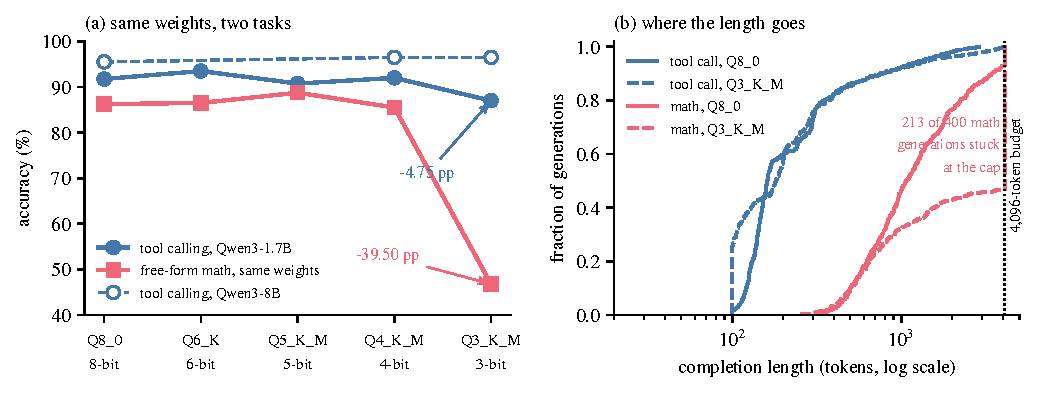
\includegraphics[width=\linewidth]{../figures/fig1-ladder.pdf}
\caption{(a) Accuracy across the quantization ladder on identical weight files: tool calling on \bfcl{} and free-form mathematics on GSM8K for \qm{}, with Qwen3-8B tool calling dashed. Both floors sit at Q4\_K\_M; the free-form drop at Q3\_K\_M is about eight times the tool-calling drop. (b) Cumulative distribution of per-request completion length at Q8\_0 and Q3\_K\_M for each task, from the result files. Tool calls are short at both rungs, and shorter at Q3\_K\_M because \qtToolNoReasonThree{} of 400 skip the reasoning block, while math generations at Q3\_K\_M pile up against the 4{,}096-token budget and \qtGsmTruncThree{} of 400 reach it.}
\label{fig:ladder}
\end{figure}

\begin{table}[t]
\centering\scriptsize\setlength{\tabcolsep}{3pt}
\begin{tabular}{@{}llrrrlrrr@{}}
\toprule
Rung & Strict [95\% CI] & Lenient & Gap & vs.\ Q8\_0 & McNemar $p$ (Holm) & Median tokens & Truncated & Truncated, correct \\
\midrule
Q8\_0 & 86.25\% [82.5, 89.3] & 86.50\% & +0.25\,pp & baseline & & 1065 & 28 & 0 \\
Q6\_K & 86.50\% [82.8, 89.5] & 86.50\% & +0.00\,pp & $+$0.25\,pp & 1.000 (1.000) & 1102 & 32 & 0 \\
Q5\_K\_M & 88.75\% [85.3, 91.5] & 89.25\% & +0.50\,pp & $+$2.50\,pp & 0.164 (0.492) & 955 & 21 & 0 \\
Q4\_K\_M & 85.50\% [81.7, 88.6] & 85.75\% & +0.25\,pp & $-$0.75\,pp & 0.736 (1.000) & 1048 & 34 & 0 \\
Q3\_K\_M & 46.75\% [41.9, 51.6] & 46.75\% & +0.00\,pp & $-$39.50\,pp & $<$0.0001 (\textbf{$<$0.0001}) & 4096 & 213 & 29 \\
\bottomrule
\end{tabular}

\caption{The free-form control, GSM8K, \qm{}, $n=400$ per rung, identical weight files to Table~\ref{tab:ladder}. Brackets are Wilson 95\% intervals on the strict score. Gap is lenient minus strict. $p$ is McNemar's exact test against Q8\_0 with the Holm-adjusted value in brackets, bold where below 0.05. Median tokens is the completion length; the budget was 4{,}096. Truncated counts generations that reached the budget, and the last column those among them that had already committed to the correct answer.}
\label{tab:gsm8k}
\end{table}

\textbf{H3 as written.} The hypothesis file said the drop measured by AST matching would be smaller than the drop measured on the free-form set under strict extraction by at least five points. At Q3\_K\_M the two drops are \qtDropThree{} and \qtGsmDropThree{} points, a difference of \qtHthreeDiff{}, so H3 holds as written; at the rungs above Q3\_K\_M both drops are within the instrument's noise and the hypothesis has nothing to bound. What H3 was meant to bound, how much of a published free-form drop is the parser, is a separate observation that the file did not register: the gap between strict and lenient scoring is at most \qtGsmGapMax{} points at any rung. Once the strict extractor accepts the commitment format reasoning models emit, the failures at Q3\_K\_M are generations with no committed answer, or a wrong one, not answers a parser failed to find. The mechanism is truncation, not extraction. Earlier drafts of this paper scored H3 on that gap and reported it as a null; the registered statistic is the one above.

\textbf{The budget.} A collapse driven by truncation could be an artefact of the 4{,}096-token cap rather than of the weights. We re-ran the \qtBudOf{} Q3\_K\_M generations that hit the cap with a budget of 16{,}384 tokens, four times the original. Of the \qtBudN{} that completed without a server error, \qtBudStillCap{} (\qtBudStillCapPct{}\%) hit the larger cap as well, and \qtBudRecovered{} (\qtBudRecoveredPct{}\%) reached a correct answer. Given four times the room, the three-bit model mostly keeps thinking. A larger budget converts most of the truncations into longer truncations.

\subsection{Across models, strict and coerced}
\label{sec:models}

Table~\ref{tab:models} gives every model at Q8\_0, Q4\_K\_M and Q3\_K\_M under both verdicts; the \qm{} rows repeat Table~\ref{tab:ladder}. On Qwen3-8B there is no cliff. Q3\_K\_M scores \qtAccEightBThree{}\% [\qtCiEightBThree{}] against \qtAccEightBEight{}\% [\qtCiEightBEight{}] at Q8\_0, a difference of \qtDeltaEightBThree{} points at $p=\qtPEightBThree{}$, and Q4\_K\_M is likewise indistinguishable from the baseline. Qwen3-14B repeats the pattern: \qtAccFourteenBEight{}\% at Q8\_0, \qtAccFourteenBFour{}\% at Q4\_K\_M and \qtAccFourteenBThree{}\% at Q3\_K\_M, with the Q3\_K\_M difference at \qtDeltaFourteenBThree{} points and $p=\qtPFourteenBThree{}$. On this family the three-bit cliff that binds at 1.7B has moved below the ladder by 8B and stays there at 14B, which is the direction the free-form literature reports for larger models and is now shown for the call itself at two sizes. The coerced columns for the three Qwen3 models are identical to the strict ones, because none of their strict failures is a quoted value of the right type or an undecoded JSON call. Both Llama models are single runs at $n=\qtNEightB{}$, and their intervals are correspondingly wider than the 1.7B ones.

Table~\ref{tab:fourbit} puts a size on ``no detectable loss'' at four bits. For each model it gives the paired Q8\_0 to Q4\_K\_M difference with its 95\% interval and the minimum detectable difference at the observed discordance. Under the coerced verdict no lower interval end is below $\qtFourBitLoCoerced{}$ points and the minimum detectable difference runs from \qtFourBitMdeMin{} to \qtFourBitMdeMax{} points; under the strict verdict the widest case is Llama-3.2-3B at $\qtFourBitLoStrict{}$. So four bits shows no loss larger than about three to five points on any model here, depending on the model and the verdict, and the design cannot exclude a loss of that size on the $n=\qtNEightB{}$ models.

\begin{table}[t]
\centering\scriptsize\setlength{\tabcolsep}{2.5pt}
\begin{tabular}{@{}llrlrrlrr@{}}
\toprule
Model & Rung & $n$ & Strict [95\% CI] & vs.\ Q8\_0 & $p$ & Coerced [95\% CI] & vs.\ Q8\_0 & $p$ \\
\midrule
Qwen3-1.7B & Q8\_0 & 400 & 91.75\% [88.6, 94.1] & baseline &  & 91.75\% [88.6, 94.1] & baseline &  \\
Qwen3-1.7B & Q4\_K\_M & 400 & 92.00\% [88.9, 94.3] & $+$0.25\,pp & 1.000 & 92.00\% [88.9, 94.3] & $+$0.25\,pp & 1.000 \\
Qwen3-1.7B & Q3\_K\_M & 400 & 87.00\% [83.3, 89.9] & $-$4.75\,pp & \textbf{0.004} & 87.00\% [83.3, 89.9] & $-$4.75\,pp & \textbf{0.004} \\
\midrule
Qwen3-8B & Q8\_0 & 200 & 95.50\% [91.7, 97.6] & baseline &  & 95.50\% [91.7, 97.6] & baseline &  \\
Qwen3-8B & Q4\_K\_M & 200 & 96.50\% [93.0, 98.3] & $+$1.00\,pp & 0.625 & 96.50\% [93.0, 98.3] & $+$1.00\,pp & 0.625 \\
Qwen3-8B & Q3\_K\_M & 200 & 96.50\% [93.0, 98.3] & $+$1.00\,pp & 0.688 & 96.50\% [93.0, 98.3] & $+$1.00\,pp & 0.688 \\
\midrule
Qwen3-14B & Q8\_0 & 200 & 96.00\% [92.3, 98.0] & baseline &  & 96.00\% [92.3, 98.0] & baseline &  \\
Qwen3-14B & Q4\_K\_M & 200 & 96.00\% [92.3, 98.0] & $+$0.00\,pp & 1.000 & 96.00\% [92.3, 98.0] & $+$0.00\,pp & 1.000 \\
Qwen3-14B & Q3\_K\_M & 200 & 96.50\% [93.0, 98.3] & $+$0.50\,pp & 1.000 & 96.50\% [93.0, 98.3] & $+$0.50\,pp & 1.000 \\
\midrule
Llama-3.2-3B & Q8\_0 & 200 & 92.00\% [87.4, 95.0] & baseline &  & 93.50\% [89.2, 96.2] & baseline &  \\
Llama-3.2-3B & Q4\_K\_M & 200 & 88.00\% [82.8, 91.8] & $-$4.00\,pp & \textbf{0.021} & 91.00\% [86.2, 94.2] & $-$2.50\,pp & 0.125 \\
Llama-3.2-3B & Q3\_K\_M & 200 & 86.50\% [81.1, 90.6] & $-$5.50\,pp & \textbf{0.007} & 91.00\% [86.2, 94.2] & $-$2.50\,pp & 0.180 \\
\midrule
Llama-3.1-8B & Q8\_0 & 200 & 50.00\% [43.1, 56.9] & baseline &  & 92.00\% [87.4, 95.0] & baseline &  \\
Llama-3.1-8B & Q4\_K\_M & 200 & 63.00\% [56.1, 69.4] & $+$13.00\,pp & \textbf{$<$0.0001} & 90.50\% [85.6, 93.8] & $-$1.50\,pp & 0.453 \\
Llama-3.1-8B & Q3\_K\_M & 200 & 71.50\% [64.9, 77.3] & $+$21.50\,pp & \textbf{$<$0.0001} & 85.00\% [79.4, 89.3] & $-$7.00\,pp & \textbf{0.003} \\
\bottomrule
\end{tabular}

\caption{Tool calling across five models on \texttt{simple\_python}, under the strict \bfcl{} verdict and the type-coerced verdict of \S\ref{sec:problem}. \qm{} at $n=\qtN{}$ (rows from Table~\ref{tab:ladder}); the other four at $n=\qtNEightB{}$, one run per rung. Brackets after an accuracy are Wilson 95\% intervals. Each model is compared against its own Q8\_0 by McNemar's exact test; $p$ is followed by the Holm-adjusted $p$ within that model's family, in bold where the adjusted value is below 0.05. Lost/gained are for the coerced verdict.}
\label{tab:models}
\end{table}

\begin{table}[t]
\centering\footnotesize\setlength{\tabcolsep}{3.5pt}
\begin{tabular}{@{}llrrrlrr@{}}
\toprule
Model & Verdict & $n$ & Lost & Gained & Difference [95\% CI] (pp) & $p$ (Holm) & MDD (pp) \\
\midrule
Qwen3-1.7B & strict = coerced & 400 & 13 & 14 & $+$0.25 [$-$2.3, $+$2.8] & 1.000 (1.000) & 3.6 \\
Qwen3-8B & strict = coerced & 200 & 1 & 3 & $+$1.00 [$-$1.2, $+$3.2] & 0.625 (1.000) & 2.8 \\
Qwen3-14B & strict = coerced & 200 & 3 & 3 & $+$0.00 [$-$2.6, $+$2.6] & 1.000 (1.000) & 3.4 \\
Llama-3.2-3B & strict & 200 & 9 & 1 & $-$4.00 [$-$7.1, $-$0.8] & 0.021 (0.064) & 4.4 \\
Llama-3.2-3B & coerced & 200 & 6 & 1 & $-$2.50 [$-$5.2, $+$0.2] & 0.125 (0.250) & 3.7 \\
Llama-3.1-8B & strict & 200 & 3 & 29 & $+$13.00 [$+$7.6, $+$18.2] & $<$0.0001 (\textbf{$<$0.0001}) & 7.9 \\
Llama-3.1-8B & coerced & 200 & 2 & 2 & $+$0.00 [$-$2.2, $+$2.2] & 1.000 (1.000) & 2.8 \\
\bottomrule
\end{tabular}

\caption{The four-bit bound. For each model, the paired difference between Q4\_K\_M and Q8\_0 with the adjusted Wald 95\% interval of \citet{agresti2005paired}, the McNemar $p$ with the Holm-adjusted value in brackets, and the minimum detectable difference (MDD): the smallest loss the test would detect at $\alpha=0.05$ with 80\% power at the discordance observed on that model \citep{connor1987paired}. For the Qwen3 models the coerced verdict equals the strict one.}
\label{tab:fourbit}
\end{table}

\subsection{A second family}
\label{sec:family}

The Qwen3 pattern does not transfer to the Llama models, and the two verdicts disagree about how much of what happens is capability. Under the strict checker Llama-3.2-3B loses \qtDropLlamaThreeBFour{} points at Q4\_K\_M ($p=\qtPLlamaThreeBFour{}$, \qtLostLlamaThreeBFour{} lost against \qtGainedLlamaThreeBFour{} gained) and \qtDropLlamaThreeBThree{} at Q3\_K\_M ($p=\qtPLlamaThreeBThree{}$). Within this model's family of four tests the Holm-adjusted values are \qtPHolmLlamaThreeBFour{} and \qtPHolmLlamaThreeBThree{}, so under strict scoring its cliff rung is Q3\_K\_M, and the four-bit loss is suggestive, from one run, and needs a repeat before it is read as a cliff. Under the coerced checker the same runs lose \qtCoercedDropLlamaThreeBFour{} and \qtCoercedDropLlamaThreeBThree{} points, at $p=\qtCoercedPLlamaThreeBFour{}$ and $p=\qtCoercedPLlamaThreeBThree{}$, and the model has no cliff rung on the ladder. The difference is in Table~\ref{tab:llama}: of its strict failures, \qtCoercibleLlamaThreeBEight{} at Q8\_0, \qtCoercibleLlamaThreeBFour{} at Q4\_K\_M and \qtCoercibleLlamaThreeBThree{} at Q3\_K\_M are the right value in a quoted string, so the strict loss overstates the loss in call correctness: \qtDropLlamaThreeBFour{} against \qtCoercedDropLlamaThreeBFour{} points at Q4\_K\_M and \qtDropLlamaThreeBThree{} against \qtCoercedDropLlamaThreeBThree{} at Q3\_K\_M, the remainder being a change in how the compressed weights type their arguments.

Llama-3.1-8B is the extreme case. Its Q8\_0 weights score \qtAccLlamaEightBEight{}\% under the strict checker; Q4\_K\_M and Q3\_K\_M score \qtAccLlamaEightBFour{}\% and \qtAccLlamaEightBThree{}\%, both at $p<0.0001$ against Q8\_0, an inversion of the expected order. Table~\ref{tab:llama} gives the reason in two parts. Of the \qtFailsLlamaEightBEight{} Q8\_0 strict failures, \qtTypeErrLlamaEightBEight{} are type errors, and \qtCoercibleLlamaEightBEight{} of the \qtFailsLlamaEightBEight{} pass the checker once the quoted value is parsed: the model names the right function and the right value and writes the number in quotes, as in \texttt{\{"base": "10", "height": "5"\}} for a triangle with base 10 and height 5. A quoted number appears in \qtQuotedNumLlamaEightBEight{} of \qtNEightB{} Q8\_0 outputs, \qtQuotedNumLlamaEightBFour{} at Q4\_K\_M and \qtQuotedNumLlamaEightBThree{} at Q3\_K\_M, while outputs with a bare number rise from \qtBareNumLlamaEightBEight{} to \qtBareNumLlamaEightBThree{}. The second part is the handler. \bfcl{}'s decoder rejects \qtDecodeErrLlamaEightBEight{}, \qtDecodeErrLlamaEightBFour{} and \qtDecodeErrLlamaEightBThree{} outputs down the ladder; \qtDecodeJsonLlamaEightBEight{}, \qtDecodeJsonLlamaEightBFour{} and \qtDecodeJsonLlamaEightBThree{} of those are well-formed JSON tool calls in Meta's format that contain a bare \texttt{true} or \texttt{false}, which the handler's \texttt{eval()} does not accept (\S\ref{sec:scoring}). The same weights write a bare boolean in \qtBareBoolLlamaEightBEight{}, \qtBareBoolLlamaEightBFour{} and \qtBareBoolLlamaEightBThree{} outputs and a quoted one in \qtQuotedBoolLlamaEightBEight{}, \qtQuotedBoolLlamaEightBFour{} and \qtQuotedBoolLlamaEightBThree{}, so the rise in decode failures is the same typing habit seen through the parser. The coerced verdict, which parses the quoted values and re-reads the JSON calls, restores the expected order and flattens it: \qtCoercedAccLlamaEightBEight{}\% [\qtCoercedCiLlamaEightBEight{}], \qtCoercedAccLlamaEightBFour{}\% [\qtCoercedCiLlamaEightBFour{}] and \qtCoercedAccLlamaEightBThree{}\% [\qtCoercedCiLlamaEightBThree{}] down the ladder, a difference of \qtCoercedDeltaLlamaEightBFour{} points at Q4\_K\_M (\qtCoercedLostLlamaEightBFour{} lost, \qtCoercedGainedLlamaEightBFour{} gained) and a loss of \qtCoercedDropLlamaEightBThree{} at Q3\_K\_M (\qtCoercedLostLlamaEightBThree{} lost, \qtCoercedGainedLlamaEightBThree{} gained, $p=\qtCoercedPLlamaEightBThree{}$). Neither is a detectable loss. Earlier drafts of this paper, which did not re-read the decode failures, reported a coerced loss of seven points at Q3\_K\_M on this model; most of that loss was the parser. Free-form accuracy on the same files falls \qtLlamaEightBGsmDropFour{} points at Q4\_K\_M (Holm $p=\qtLlamaEightBGsmPHolmFour{}$) and \qtLlamaEightBGsmDropThree{} at Q3\_K\_M (Holm $p=\qtLlamaEightBGsmPHolmThree{}$). Length plays no part in either Llama model: GSM8K completions have a median of \qtLlamaThreeBGsmMedTokEight{} to \qtLlamaEightBGsmMedTokEight{} tokens, and at most \qtLlamaEightBGsmTruncThree{} of 400 reach the budget at any rung, so the run-away behind the Qwen3 collapse cannot occur and the free-form losses here are ordinary precision loss.

What the second family adds is one finding and two warnings. The finding is that quantization changes argument typing before it changes call correctness: on both Llama models the count of coercible failures moves with the rung while the coerced accuracy at Q4\_K\_M does not differ from Q8\_0. The first warning is that a strict schema score can move in either direction under quantization, because it measures a formatting habit as much as a capability, and a reader given only the strict column of Table~\ref{tab:models} would conclude that compressing Llama-3.1-8B improves it by \qtDropLlamaEightBThree{} points. The second is that a checker's decode-failure count can be the checker's own parser: a reader given the failure counts but not the raw outputs would conclude that three-bit weights stop producing parseable calls, when they produce calls in the format the model was trained on that this handler does not read. Anyone scoring tool calls under compression should report the failure types, read the raw outputs behind the decode failures, and put a coerced score beside the strict one.

\begin{table}[t]
\centering\scriptsize\setlength{\tabcolsep}{2.5pt}
\begin{tabular}{@{}llrrrrlrr@{}}
\toprule
Model & Rung & Strict failures & Type errors & Decode errors & Coercible & GSM8K strict [95\% CI] & vs.\ Q8\_0 & $p$ \\
\midrule
Llama-3.2-3B & Q8\_0 & 16 & 6 & 0 & 3 & 84.00\% [80.1, 87.3] & baseline &  \\
Llama-3.2-3B & Q4\_K\_M & 24 & 10 & 0 & 6 & 81.25\% [77.1, 84.8] & $-$2.75\,pp & 0.126 \\
Llama-3.2-3B & Q3\_K\_M & 27 & 13 & 0 & 9 & 75.50\% [71.1, 79.5] & $-$8.50\,pp & \textbf{$<$0.0001} \\
\midrule
Llama-3.1-8B & Q8\_0 & 100 & 90 & 3 & 84 & 91.00\% [87.8, 93.4] & baseline &  \\
Llama-3.1-8B & Q4\_K\_M & 74 & 61 & 6 & 55 & 87.75\% [84.2, 90.6] & $-$3.25\,pp & \textbf{0.041} \\
Llama-3.1-8B & Q3\_K\_M & 57 & 32 & 14 & 27 & 83.25\% [79.3, 86.6] & $-$7.75\,pp & \textbf{$<$0.0001} \\
\bottomrule
\end{tabular}

\caption{The second family. Failure types on \texttt{simple\_python} ($n=\qtNEightB{}$ per rung, one run): strict failures, of which type errors and decode failures, the decode failures whose raw output is one well-formed JSON call, and the strict failures that pass the coerced checker. GSM8K strict accuracy, $n=400$, with Wilson 95\% intervals, each model against its own Q8\_0 by McNemar's exact test, with the Holm-adjusted $p$ in brackets.}
\label{tab:llama}
\end{table}

\subsection{Multi-turn trajectories}
\label{sec:multiturn}

The hypothesis file predicted that multi-turn trajectories, where an error in one call corrupts the state for every call after it, would degrade at least twice as fast as single calls. Table~\ref{tab:multiturn} gives \bfcl{}'s \texttt{multi\_turn\_base} on \qm{}, $n=\qtMtN{}$, which is the whole category: \qtMtAccEight{}\% at Q8\_0, \qtMtAccFour{}\% at Q4\_K\_M and \qtMtAccThree{}\% at Q3\_K\_M. Those numbers cannot be read as a property of the weights. The server for this arm ran \qtMtSlots{} slots on a \qtMtCtxSlot{}-token KV cache that the slots share, and a request whose accumulated context did not fit beside the other three was refused with ``Context size has been exceeded''; \texttt{bfcl-eval} records the refusal as the trajectory's result and the checker scores it as a failure. That happened to \qtMtCtxErrEight{}, \qtMtCtxErrFour{} and \qtMtCtxErrThree{} of the 200 trajectories at Q8\_0, Q4\_K\_M and Q3\_K\_M; a further 2, 1 and 2 ended in a handler exception on a malformed call, which is an ordinary failure, so \qtMtAbortedEight{}, \qtMtAbortedFour{} and \qtMtAbortedThree{} trajectories carry no completed run. On the trajectories that ran to completion, accuracy is \qtMtCompletedCorrectEight{} of \qtMtCompletedEight{} (\qtMtCompletedAccEight{}\%), \qtMtCompletedCorrectFour{} of \qtMtCompletedFour{} (\qtMtCompletedAccFour{}\%) and \qtMtCompletedCorrectThree{} of \qtMtCompletedThree{} (\qtMtCompletedAccThree{}\%), but the completed set at Q3\_K\_M is the third of trajectories that stayed short, so that comparison is biased in its own way. On the completed trajectories the per-request completion has a median of \qtMtReqMedEight{}, \qtMtReqMedFour{} and \qtMtReqMedThree{} tokens, and the accumulated context per request a median of \qtMtCtxMedEight{}, \qtMtCtxMedFour{} and \qtMtCtxMedThree{} tokens, a 90th percentile of \qtMtCtxPninezeroEight{}, \qtMtCtxPninezeroFour{} and \qtMtCtxPninezeroThree{}, and a maximum of \qtMtCtxMaxEight{}, \qtMtCtxMaxFour{} and \qtMtCtxMaxThree{}: no single trajectory needed the whole cache, and four together did. Whether three-bit weights push more trajectories over the limit because they generate more per turn, or because the aborts fell on them by scheduling, cannot be separated in this run. The rising 90th-percentile context points to the first; the quarter of Q8\_0 trajectories lost to the same error shows the second is large. H5 is therefore not evaluable from this run. Earlier drafts of this paper reported it as supported by a wide margin, on the all-trajectory numbers, without having noticed the aborts. The arm has to be re-run with a context each trajectory owns, one slot or a per-slot cache, before the hypothesis can be read either way.

\begin{table}[t]
\centering\scriptsize\setlength{\tabcolsep}{3pt}
\begin{tabular}{@{}lrlrrrrr@{}}
\toprule
Rung & $n$ & Accuracy [95\% CI] & vs.\ Q8\_0 & Lost/Gained & McNemar $p$ & Relative (\%) & Single call, relative (\%) \\
\midrule
Q8\_0 & 200 & 17.00\% [12.4, 22.8] & baseline & & & & \\
Q4\_K\_M & 200 & 13.50\% [9.4, 18.9] & $-$3.50\,pp & 16/9 & 0.230 & $-$20.6 & $+$0.3 \\
Q3\_K\_M & 200 & 1.50\% [0.5, 4.3] & $-$15.50\,pp & 32/1 & \textbf{$<$0.0001} & $-$91.2 & $-$5.2 \\
\bottomrule
\end{tabular}

\caption{Multi-turn tool calling, \bfcl{} \texttt{multi\_turn\_base}, \qm{}, $n=\qtMtN{}$ per rung (the whole category), one run. Accuracy over all trajectories, with Wilson 95\% intervals, as \bfcl{} scores it; McNemar's $p$ against Q8\_0 with the Holm-adjusted value in brackets. Aborted counts trajectories that ended in a server context error or a handler exception and were scored as failures; the last column is the accuracy on the trajectories that ran to completion. The rung comparison is confounded by the aborts (\S\ref{sec:multiturn}).}
\label{tab:multiturn}
\end{table}

\subsection{Does the overthinking penalty transfer}
\label{sec:penalty}

The penalty has no measurable effect. With it, \qm{} scores \qtHfourAccFour{}\% at Q4\_K\_M and \qtHfourAccThree{}\% at Q3\_K\_M, identical to the unpenalised runs to two decimals; at each rung \qtHfourLostFour{} questions flip one way and \qtHfourGainedFour{} the other, within the repeat-control range of Table~\ref{tab:repeats}. H4 predicted a loss of at least three points and there is no loss. The explanation follows from \S\ref{sec:freeform}: the penalty acts on tokens a reasoning trace emits and a tool call does not, so on a \qtToolNgenMedThree{}-token output there is almost nothing for it to act on. This agrees with the authors' own scope statement that the marker list was curated for free-form English reasoning. Both the failure they describe and the fix for it live in the reasoning trace, and the tool call contains very little of that trace.

\subsection{The hypotheses against their written thresholds}
\label{sec:hyp}

H1 (the schema breaks first) was written on schema validity, the share of outputs the checker decodes as a call, falling below 95\% of its reference value at a higher bit-width than free-form accuracy does. On \qm{} schema validity is \qtSchemaValidEight{}\% at Q8\_0 and never below \qtHoneSchemaMin{}\% at any rung, against a threshold of \qtHoneSchemaThresh{}\%, so it never triggers; free-form accuracy crosses its own 95\% line (\qtHoneGsmThresh{}\%) at Q3\_K\_M. Under the registered statistic the schema does not break at all on this ladder, and under AST accuracy both floors sit at Q4\_K\_M. H1 is not supported under either reading.

H2 (failure mode shifts) said the share of failures that are structural, meaning no call decoded, a wrong function name, a wrong number of calls or a missing parameter, rather than semantic, meaning a wrong value or type, would rise by at least 15 points from Q8\_0 to Q3\_K\_M. Table~\ref{tab:htwo} gives it for every model from \bfcl{}'s own error categories. On \qm{} it rises from \qtStructShareEight{}\% to \qtStructShareThree{}\%, \qtHtwoDelta{} points, below the threshold; on Qwen3-14B and Llama-3.2-3B it does not rise; on Qwen3-8B it rises by \qtHtwoDeltaEightB{} points on \qtFailsEightBThree{} failures; on Llama-3.1-8B it rises by \qtHtwoDeltaLlamaEightB{} points by \bfcl{}'s categories and by \qtHtwoDeltaJsonLlamaEightB{} once the \qtDecodeJsonLlamaEightBThree{} JSON calls are decoded. The hallucinated-function rate, the third registered metric, is at most \qtHallucFnThree{}\% on any rung of any model (\qtWrongNameThree{} of \qtN{} calls on \qm{} at Q3\_K\_M, each a corrupted spelling of the right name). H2 is not supported on the primary model.

H3 holds as written (\S\ref{sec:freeform}), and on the Llama models too: the coerced AST drop at Q3\_K\_M is smaller than the strict free-form drop by \qtLlamaThreeBHthreeDiff{} points on Llama-3.2-3B and \qtLlamaEightBHthreeDiff{} on Llama-3.1-8B. H4 predicted a loss of at least three points under the penalty and found \qtHfourDropThree{} (\S\ref{sec:penalty}). H5 cannot be evaluated from this run (\S\ref{sec:multiturn}).

\begin{table}[t]
\centering\footnotesize\setlength{\tabcolsep}{4pt}
\begin{tabular}{@{}lrrrrrrr@{}}
\toprule
Model & Failures Q8\_0 & Structural & Share (\%) & Failures Q3\_K\_M & Structural & Share (\%) & Change (pp) \\
\midrule
Qwen3-1.7B & 33 & 3 & 9.1 & 52 & 8 & 15.4 & $+$6.3 \\
Qwen3-8B & 9 & 0 & 0.0 & 7 & 3 & 42.9 & $+$42.9 \\
Qwen3-14B & 8 & 0 & 0.0 & 7 & 0 & 0.0 & $+$0.0 \\
Llama-3.2-3B & 16 & 4 & 25.0 & 27 & 4 & 14.8 & $-$10.2 \\
Llama-3.1-8B & 100 & 3 & 3.0 & 57 & 14 & 24.6 & $+$21.6 \\
\bottomrule
\end{tabular}

\caption{H2 as written: the structural share of strict failures at Q8\_0 and Q3\_K\_M per model, from \bfcl{}'s error categories. Structural is decode failure, wrong function name, wrong call count or missing parameter; the rest are wrong values or types. The threshold was a rise of 15 points. On Llama-3.1-8B \qtDecodeJsonLlamaEightBThree{} of the \qtStructLlamaEightBThree{} structural failures at Q3\_K\_M are JSON calls the handler did not decode.}
\label{tab:htwo}
\end{table}

\section{Discussion}

Of the five hypotheses, one held as written, three did not, and one cannot be read from this run. H1, that the schema would break first, reversed under both its registered statistic and AST accuracy. H2, that failures would turn structural, moved \qtHtwoDelta{} points on the primary model against a threshold of 15. H3, that the AST drop would be smaller than the strict free-form drop by at least five points, held by \qtHthreeDiff{} points; the separate question it was meant to bound, how much of a free-form drop is the parser, has the answer \qtGsmGapMax{} points at most. H4, that the overthinking penalty would cost schema compliance, found a change of \qtHfourDropThree{} points. H5, on multi-turn amplification, is confounded by a shared server cache and is reported as such rather than as the wide-margin support earlier drafts claimed.

The tool-calling floor is a property of the model, not of the format. At four bits no model shows a loss larger than the intervals in Table~\ref{tab:fourbit} allow, which is three to five points depending on the model and the verdict, and the coerced verdict at Q4\_K\_M sits within \qtCoercedDropLlamaThreeBFour{} points of Q8\_0 on every model; three bits costs \qm{} \qtDropThree{} points and Llama-3.2-3B \qtDropLlamaThreeBThree{} strict points, and costs Qwen3-8B, Qwen3-14B and Llama-3.1-8B nothing detectable at these sample sizes. The mechanism that damages free-form reasoning at three bits on Qwen3, a chain of thought that runs past its budget, does not reach a single tool call because the call is over long before the run-away starts.

On the measurement itself, three points for another group. First, report the failure types. The Llama-3.1-8B inversion in the strict column of Table~\ref{tab:models} would read as a broken harness to anyone who did not see Table~\ref{tab:llama}, and it took a re-score of the existing files, not a new run, to show that \qtCoercibleLlamaEightBEight{} of \qtFailsLlamaEightBEight{} failures were the right number in quotes. Second, read the raw outputs behind a checker's decode failures: \qtDecodeJsonLlamaEightBThree{} of \qtDecodeErrLlamaEightBThree{} here were the checker's parser, and a hypothesis about structural failure (H2) would have been declared supported on that model without the reading. Third, measure the instrument, and read its logs. Three runs with the same weights moved by at most \qtMaxRepRange{} points (Table~\ref{tab:repeats}); without that figure none of the other differences could be attributed to anything. The multi-turn arm is the counter-example: a server error recorded in every result file went unread through two drafts, and the arm's headline number was the error rate.

\textbf{Practical reading.} For anyone deploying an agent on a laptop: four bits shows no single-call loss larger than about three to five points on any model measured here, which is the bound the sample sizes give and not a guarantee of zero; three bits costs \qm{} and, under strict scoring, Llama-3.2-3B; the bit-width should be measured on the model being shipped rather than assumed from another family; a strict schema score should be read together with a coerced one and the failure types; and the serving configuration, not only the weights, decides whether a multi-turn agent finishes, since the multi-turn arm here was decided by a shared cache before the weights had a say. A model that emits malformed or wrong tool calls can take real actions, so agents should be tested at the exact quantization and context configuration they ship with.

\textbf{Limitations.} Three sizes of one model family and two sizes of a second, on the easiest \bfcl{} category plus one multi-turn set for \qm{} only, on one hardware platform and one inference server. The hypotheses were written in a file whose first commit postdates the first ladder, so their priority rests on the author's record. FP16 was the planned reference arm and was not run; every comparison is against Q8\_0. The ladder is one quantization family; GPTQ, AWQ and the other research methods are deliberately out of scope, and multilingual degradation is excluded because \citet{marchisio2024multilingual} already cover it. The reproducibility control was run on two rungs of one model rather than on every rung of every model, so the tolerance of \qtMaxRepRange{} points is measured on \qm{} and assumed for the other four; the Llama-3.2-3B strict result at Q4\_K\_M rests on \qtLostLlamaThreeBFour{} lost against \qtGainedLlamaThreeBFour{} gained from a single run and does not survive the within-model correction, and a repeat on that model is the second thing we would add. Four of the five models were scored on the first \qtNEightB{} items of the category, which halves their power relative to the 1.7B ladder; the minimum detectable differences in Table~\ref{tab:fourbit} are the consequence. The free-form control uses a 4{,}096-token budget; the 16{,}384-token re-run shows that a larger budget recovers few of the \qtGsmTruncThree{} truncated generations. The Llama-3.1-8B typing habit was diagnosed from the score files, the raw outputs and the published prompting-mode number, not by re-running the weights on a second server or through a second tool-template path; that cross-check is the first thing we would add. The overthinking penalty is one fixed $\lambda$ rather than the authors' tuned value. The multi-turn arm is confounded by a shared KV cache and has to be re-run with a per-trajectory context; until then it says nothing about the weights. Latency was recorded for the 1.7B ladder only.

\section{Conclusions}

We expected a function signature, having no slack, to be the first thing quantization breaks. On the deployed format, scored deterministically, it was the output that held up best. For \qm{} the tool-calling floor and the free-form floor sit at the same rung, Q4\_K\_M, but the call loses \qtDropThree{} points at Q3\_K\_M where the mathematics loses \qtGsmDropThree{}, and the difference is length: three-bit weights make the chain of thought grow past the token budget, and a call is complete long before that happens. On Qwen3-8B and Qwen3-14B there is no tool-calling cliff at any rung. On the Llama family the strict score moves in both directions because compression changes how the models type their arguments, and part of what the checker reports as decode failure is its own parser; scored on the parsed value, four bits costs neither Llama model detectable accuracy and three bits costs Llama-3.1-8B \qtCoercedDropLlamaEightBThree{} points, not detectable at $n=\qtNEightB{}$. A fair extractor changes at most \qtGsmGapMax{} points, and a penalty designed for reasoning traces finds little to act on in a call. The bit-width an agent can tolerate has to be measured on the model being shipped, with the bound the sample size gives stated beside the result, and the damage quantization does to long reasoning does not carry over to the tool call.

\section*{Additional Information and Declarations}

\textbf{Competing Interests.} The author is employed full time as a software engineer at Amazon (2022 to present). Amazon had no involvement in this work, which was done independently, on the author's own hardware and time, and the work is not affiliated with that employer; none of the models, quantization tools, benchmarks or inference servers evaluated is an Amazon product. The author has no financial or other interest in any of them, and none of their developers was involved in the study.

\textbf{Author Contributions.} Akshay Kumar conceived and designed the experiments, performed the experiments, analyzed the data, prepared figures and tables, authored and reviewed drafts of the article, and approved the final draft.

\textbf{Funding.} The author received no funding for this work. All computation ran on the author's own hardware.

\textbf{Use of generative AI.} A large language model coding assistant (Claude Code, Anthropic) was used to draft run scripts and analysis code, to draft and revise text, and to check citations against their sources; the lab notebook in the repository records which entries were written with it. The author reviewed every script, number and sentence and is responsible for the content.

\textbf{Preprint.} No preprint of this manuscript is public. An earlier version was submitted to arXiv on 24 September 2026 and was not accepted for announcement; it is not available anywhere.

\textbf{Data Availability.} The code, run scripts, every raw \bfcl{} result and score file, every GSM8K generation, the server logs, the hypothesis file and the dated lab notebook are available at \url{https://github.com/akshayaggarwal99/quant-tool-calling} under the MIT licence, at the release tag \texttt{v1.3-peerj}, which is the version this paper describes. An archive of that tag is deposited at Zenodo, DOI 10.5281/zenodo.XXXXXXX (reserved; to be activated on acceptance). The GGUF weight files are not included; the scripts rebuild them from the published FP16 checkpoints.

\bibliographystyle{plainnat}
\bibliography{../refs}
\end{document}
